% Chapter 3

\chapter{Galaxy Distributions} % Write in your own chapter title
\label{Chapter:GalDist}
\lhead{Chapter 3. \emph{Distributions}} % Write in your own chapter title to set the page header

\section{Background}
%What do we know about the distributions of galaxies
%Why important physics is encoded in galaxy distributions
%What is the current state of the art in galaxy distributions 
\section{Halo Structure and Dynamical Friction}

%this should simply be a refresher and re-communicate the required points from chapter 2

\section{Abundance Matching and Stellar Mass functions}
%show how stellar mass functions create different abundance matching results
\section{Multi-Epoch Distributions of Satellite Galaxies}
%Introduce the basic distribution plot with 'best fit' from the PhD

When computing the distribution of satellites as a function of parent halo mass we will show both full number densities, as well as fractional distributions to better highlight the ``skewness'' of the predicted distributions with respect to the data. The latter will be simply computed as
\begin{equation}
\label{eqn:FracPlot}
F(dM_h) = \frac{N(>10^x)|_{dM_h}}{N(x)},
\end{equation} 
where $N(>10^{x})$ is the total number (density) of satellites above a threshold stellar mass $x= \log M_{*}$, and the $N(>10^{x})|_{dM_h}$ is the number of these that reside within the halo mass bin $[M_h, M_h+dM_h]$.

\begin{figure}[h]
	\centering
	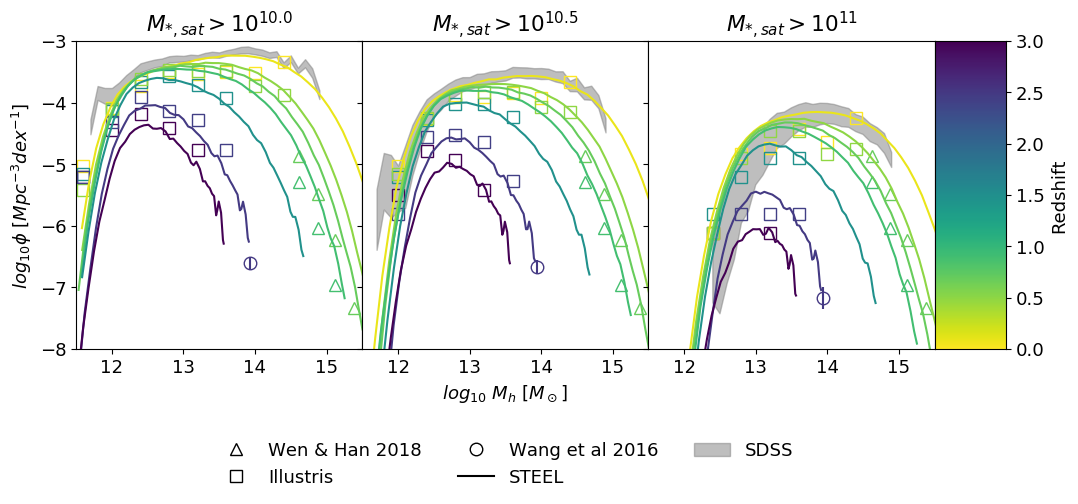
\includegraphics[width = \linewidth]{Figures/Chapter3/HighzClusters.png}
    \caption{The number-density distribution of satellites per parent halo mass predicted from \textsc{steel}, using the PyMorph SMHM relation, at multiple redshift epochs (solid lines). The grey band is the data from SDSS at redshift $z=0.1$. Also included are the high redshift cluster data from \citet{Wang2016DiscoveryZ=2.506} (circles) and \citet{Wen2018ARedshifts} (triangles). I also compare to the outputs from the Illustris simulation using the TNG100 data (crosses). Each data point and line are given a colour associated to their redshift (the bar on the right provides the color coding key).}
	\label{fig:Sat_Dist_High_z}
\end{figure}
%Show the various impact of SMHM relationships.

%Make plot showing how the distribution of satellites shifts based on two SMHM relations

%show stripping/SF routines and their effects:REMEMBER this is discussed elsewhere in detail don't write it twice.

\begin{figure}
	\centering
	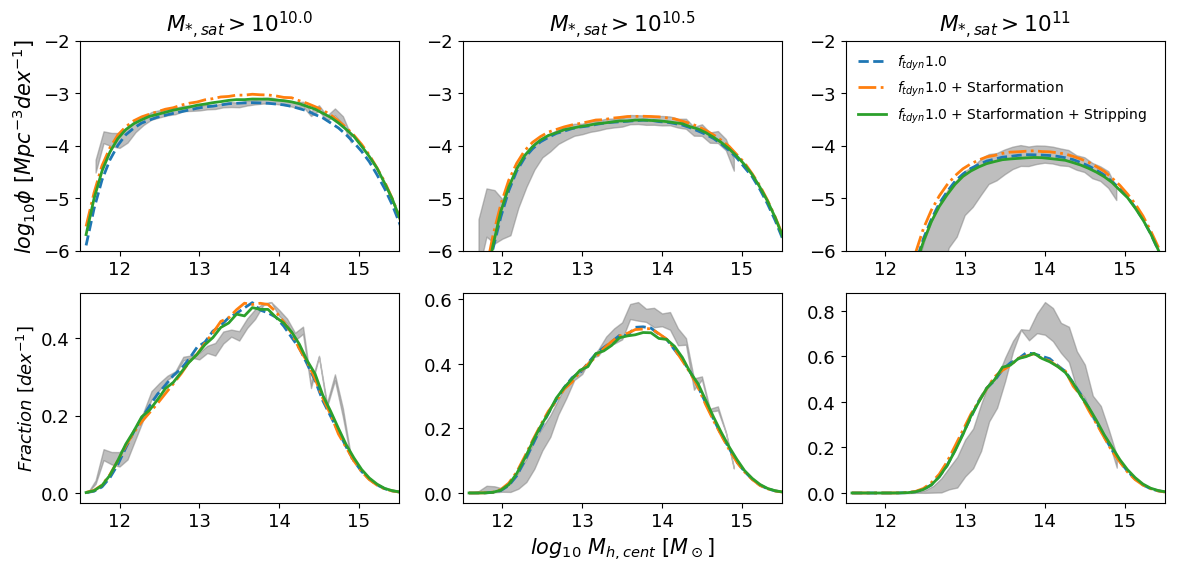
\includegraphics[width = \linewidth]{Figures/Chapter3/Sat_Dist_SF_Strip.png}
	\caption{Satellite distributions in parent haloes generated from the model are compared to those observed in SDSS (grey band). Columns from left to right show increasing satellite stellar mass cuts as labelled. The top row shows the number density of satellites expected to be found in each parent halo mass. The bottom row shows the fractional distribution described by Equation \ref{eqn:FracPlot}. The models shown all have $f_{tdyn} = 1.0$ and are the reference 'frozen model' (dashed line), starformation only (dot dashed line) and starformation and stripping (solid line). The width of the grey band corresponds to a 10\% uncertainty in satellite stellar masses.}
	\label{fig:Sat_Dist_SF_Strip}
\end{figure}


%Show the dynamical friction model and how that actually impacts the distribution.

\begin{figure}[h]
	\centering
	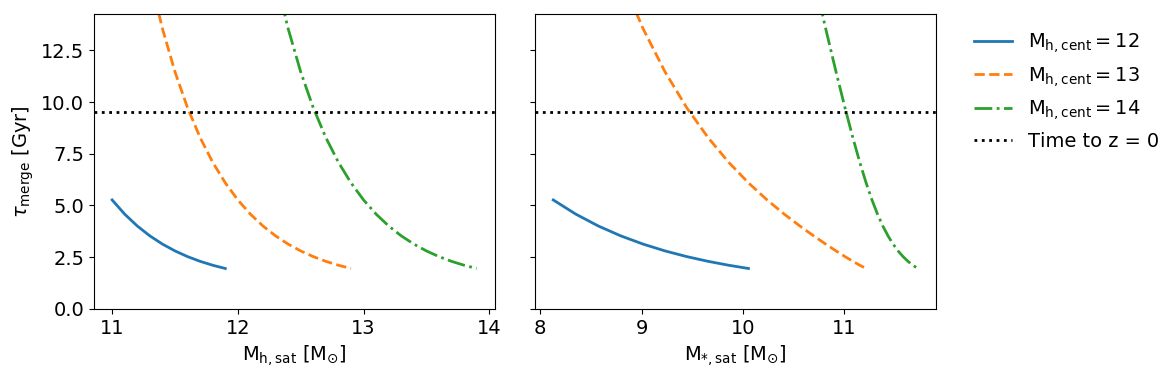
\includegraphics[width = \linewidth]{Figures/Chapter3/Tdyn_M.png}
	\caption{I show the percentage of satellites observed at a $z = 0.1$ as a function of their redshift of accretion $z > 0$. It can be seen that massive satellites observed at $z = 0.1$ are accreted more recently than smaller satellites. At $z = 0.5$ less that 50\% of the total satellites observed at $z = 0.1$ have been accreted, and at $z = 0.1$ this falls to less than 20\%. }
	\label{fig:Tdyn_M}
\end{figure}

\begin{figure}[h]
	\centering
	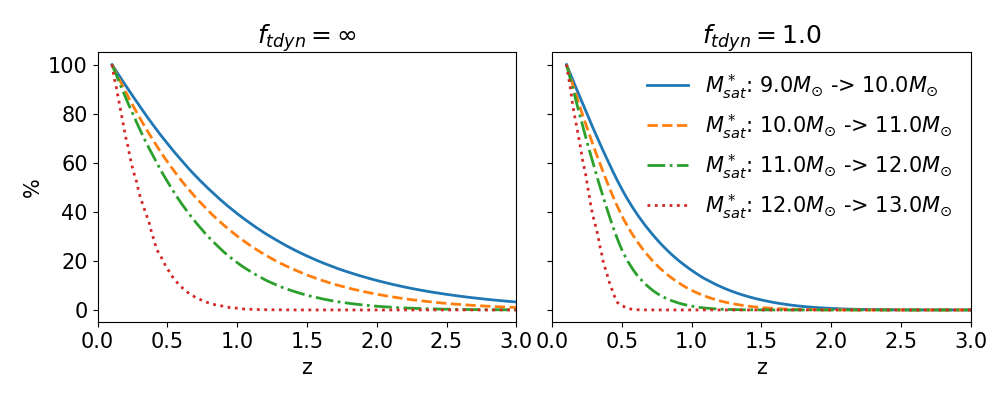
\includegraphics[width = \linewidth]{Figures/Chapter3/AccretedSatellitePercentage.png}
	\caption{I show the percentage of satellites observed at a $z = 0.1$ as a function of their redshift of accretion $z > 0$. It can be seen that massive satellites observed at $z = 0.1$ are accreted more recently than smaller satellites. At $z = 0.5$ less that 50\% of the total satellites observed at $z = 0.1$ have been accreted, and at $z = 0.1$ this falls to less than 20\%. }
	\label{fig:AccretionTime}
\end{figure}

\begin{figure}[h]
	\centering
	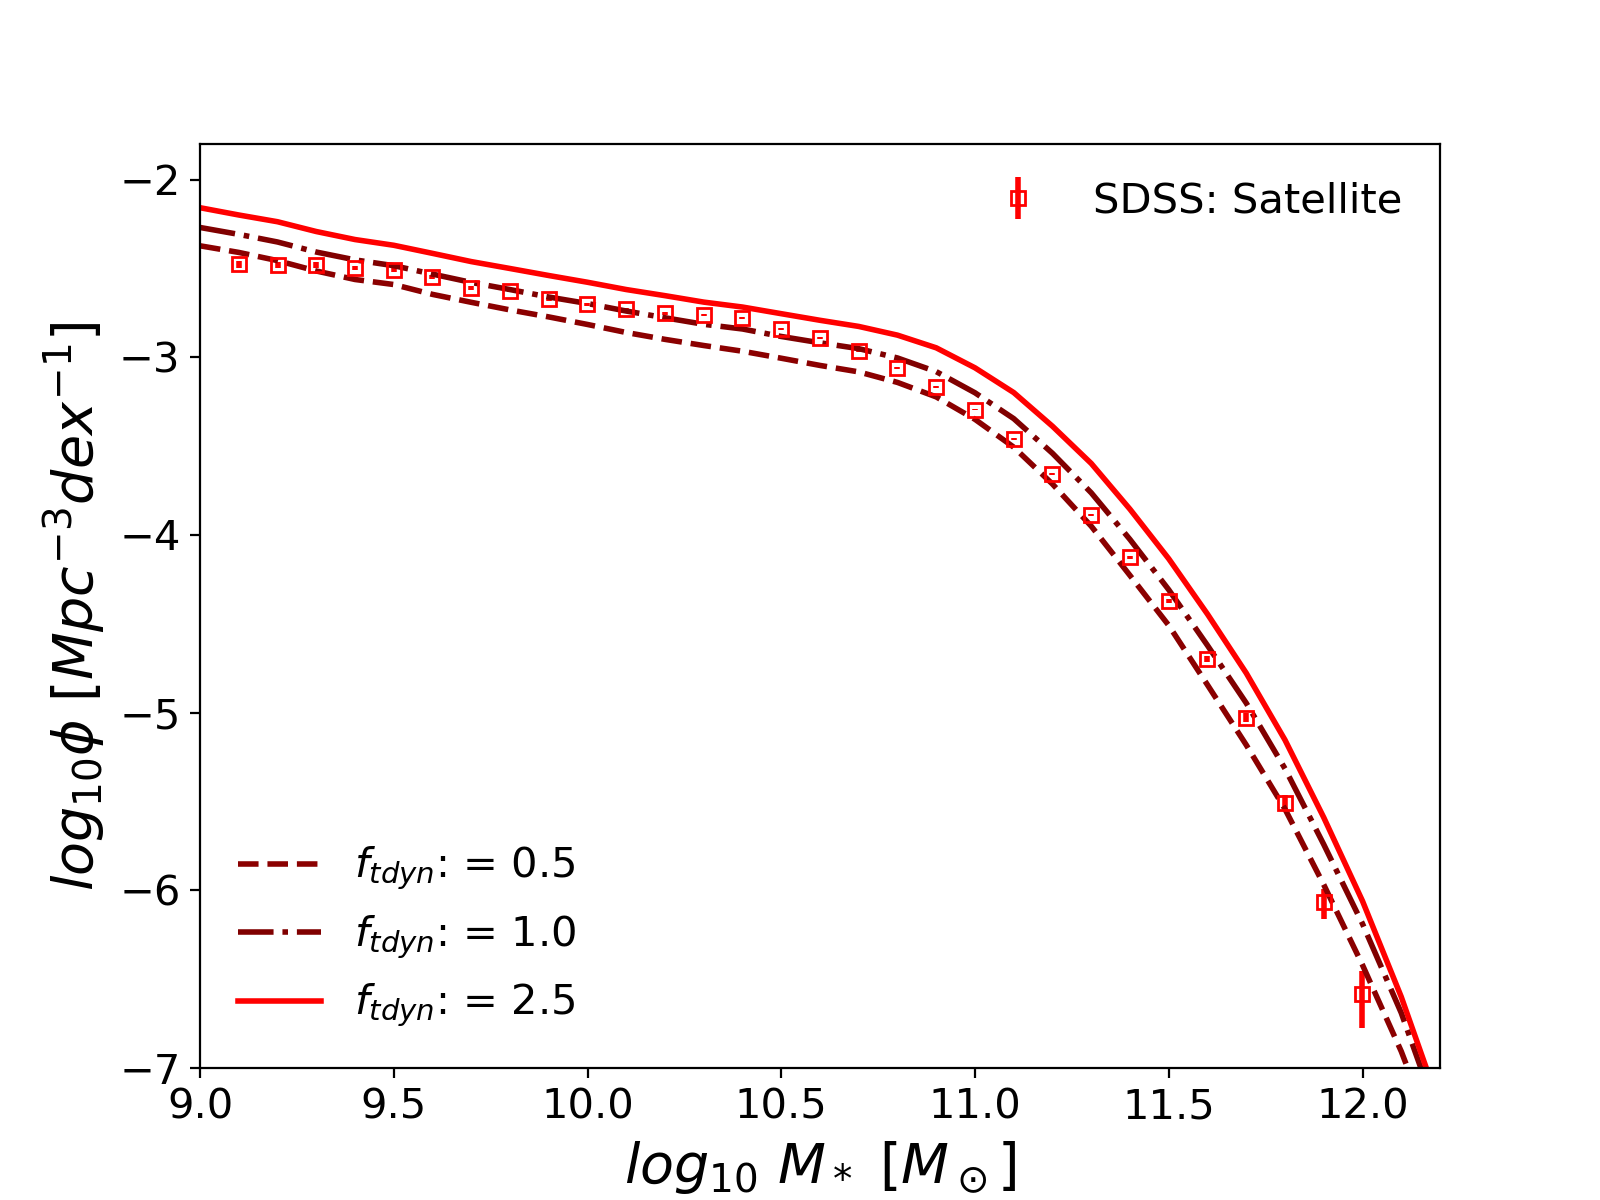
\includegraphics[width = \linewidth]{Figures/Chapter3/Tdyn_SMF.png}
	\caption{Satellite stellar mass functions generated by the model compared to SDSS data (open squares). The solid, dot dashed, and dashed lines show $f_{tdyn} = 0.5, 1.0,$ and $2.5$ respectively.}
	\label{fig:SMF_Tdyn}
\end{figure}

\begin{figure}[h]
	\centering
	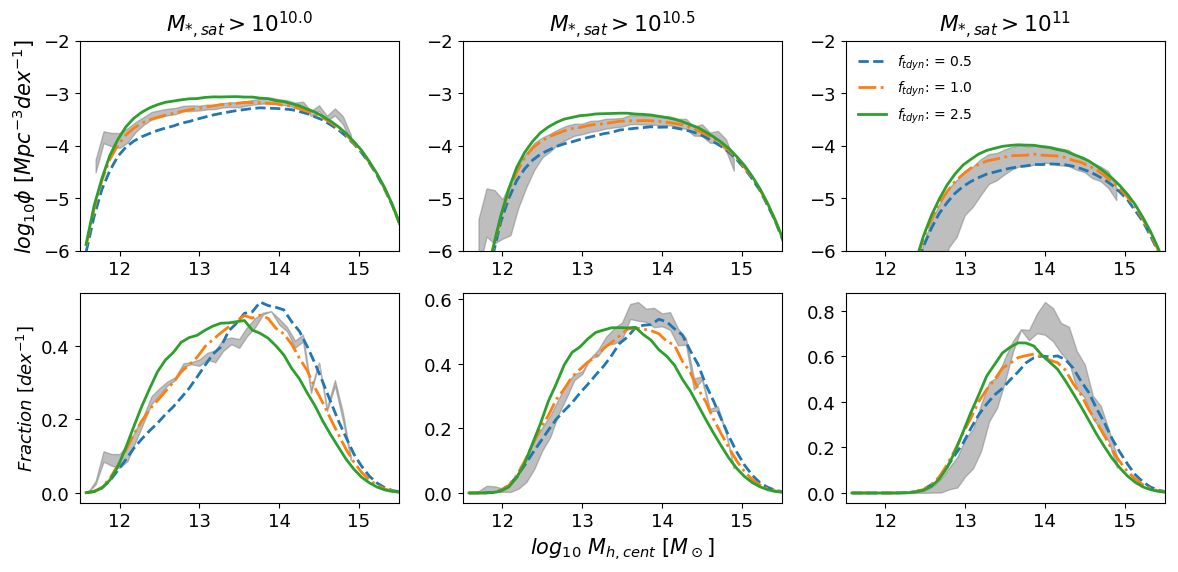
\includegraphics[width = \linewidth]{Figures/Chapter3/Tdyn_Sat_Dist.png}
	\caption{Satellite distributions in parent haloes generated from the model are compared to those observed in SDSS (grey band). Columns from left to right show increasing satellite stellar mass cuts as labelled. The top row shows the number density of satellites expected to be found in each parent halo mass. The bottom row shows the fractional distribution described by Equation \ref{eqn:FracPlot}. The dashed, dot dashed, and solid lines show $f_{tdyn} = 0.5, 1.0,$ and $2.5$ respectively. The width of the grey band corresponds to a 10\% uncertainty in satellite stellar masses.}
	\label{fig:Sat_Dist_Tdyn}
\end{figure}